% https://stackoverflow.com/a/65091926
\documentclass{beamer}
\usepackage{textcomp}
\usepackage{tikz}
\usetheme{Madrid}

 \usetikzlibrary{shapes,arrows, positioning, calc}  
 \usetikzlibrary{overlay-beamer-styles}
 
\tikzset{%
  block/.style    = {rounded corners, draw, thick, circle, minimum height = 3em,
    minimum width = 3em, fill = yellow!50},
  point/.style    = {coordinate}, % Input
}


\begin{document}
\begin{frame}{}
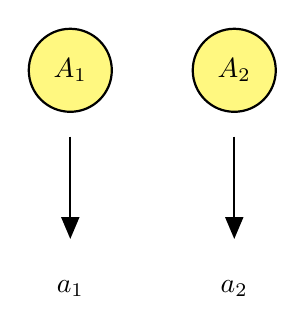
\begin{tikzpicture}[auto, thick, node distance=2cm, >=triangle 45]
\node[block] (A1) at (0,0) {$A_1$};
\node[block, right  = 1cm of A1] (A2) {$A_2$};
\node[below  = of A1, visible on=<2->] (a1) {$a_1$};
\node[below  = of A2, visible on=<2->] (a2) {$a_2$};
\draw[->] (A1.south) ++(0,-0.3) -- ++(0, -1.3);
\draw[->] (A2.south) ++(0,-0.3) -- ++(0, -1.3);
\end{tikzpicture}
\end{frame}
\end{document}
